\documentclass[12pt]{article}
\usepackage{graphicx}
\usepackage{amsmath}
%\usepackage{float}
%\usepackage{listings}
\setlength\parindent{0pt} % Removes all indentation from paragraphs

\title{Project - Elevator}
\author{Dominik Koszkul, Michal Oleszczyk, Cezary Dynak, Marek Frydrysiak }
\usepackage{geometry}
\newgeometry{tmargin=2cm, bmargin=2cm, lmargin=2cm, rmargin=2cm}
\begin{document}

\maketitle{}
%\tableofcontents{}


\section{Main concept}
	Main concept is to create two different programs (one for implementation of controller system and the second one for implementation of elevators simulation). Programs should be independent. That means they should use some general protocol for communication, and should work fine with any other external programs which also use that specified protocol. Both programs start with set of parameters: number of elevators and number of floors supported by any of them. Number of floor does not need to be the same for different elevators. Our elevator controller and simulation do not support underground floors.
\newline
\newline
Assumption: at the very beginning all elevators are in state: closed door on floor 0 (ground floor). Controller remembers current state of all elevators in anytime.

\begin{figure}
  \centering
  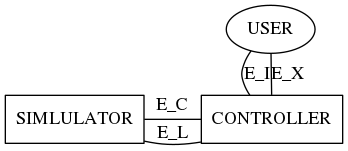
\includegraphics{img/simulator_controller.png}
  \caption{DES graph}
\end{figure}

\section{Automaton description}

\[ G = (E, S, f, \Gamma, s_0, S_M) \]

\subsection{States \(S\)}

\[ S = [W, P, Q] \]

\subsubsection{Lift states}

\[ W=[w_1, w_2, ..., w_i, ..., w_l ]\]
where:
\begin{itemize}
  \item \(l\) - number of lifts
\end{itemize}

\[ w_i = [d_i, o_i, f_i] \]
where:

\(d \in \{\text{going\_down},\text{stopped},\text{going\_up}\}\)

\(o \in \{\text{closed},\text{opened}\}\)

\(f \in \{0,1,...,i,...,n\}\)
\begin{itemize}
  \item \(i\) - next floor to be reached
  \item \(n\) - number of floors
\end{itemize}


\subsubsection{External buttons states}

\[ P = [p_1, p_2, ..., p_i, ..., p_n] \]
where:
\begin{itemize}
  \item \(n\) - number of floors
\end{itemize}

\[ p_i = [g_{i_d}, g_{i_u}] \]
where:\\
\(g_{i_d} \in \{\text{not\_pushed},\text{pushed}\}\)
\(g_{i_u} \in \{\text{not\_pushed},\text{pushed}\}\)\\


\subsubsection{Internal buttons states}
\[ Q = [q_1, q_2, ..., q_i, ..., q_l] \]
where:
\begin{itemize}
  \item \(l\) - number of lifts
\end{itemize}
\[q_i = [b_{i_0}, b_{i_1}, ..., b_{i_j}, ..., b_{i_n}] \]
\(b_{i_j} \in \{\text{not\_pushed},\text{pushed}\} \)

\newpage

\subsection{Events \(E\)}

\[ E = E^x \cup E^i \cup E^c \cup E^l \]

\subsubsection{Events from external buttons}
\[ E^x = [\text{lift\_nr},\text{button\_nr}] \]
\(\text{button\_nr} \in \{\text{button\_down},\text{button\_up}\}\)

\subsubsection{Events from internal buttons}
\[ E^i = [\text{lift\_nr},\text{button\_nr}] \]
\(\text{button\_nr} \in \{0, 1,..., n\}\)

\subsubsection{Events from controller}
\[ E^c = [\text{lift\_nr}, \text{command}] \]
\(\text{command} \in \{\text{go\_down},\text{stop},\text{go\_up},\text{close\_door},\text{open\_door}\}\)

\subsubsection{Events from lifts}
\[ E^l = [\text{lift\_nr}, \text{command}] \]
\(\text{command} \in \{\text{going\_down},\text{stopped},\text{going\_up},\text{closed},\text{opened}\}\)

\subsection{Transition function\(f(s,e)\)}

\subsubsection{Events from external buttons}
\[
  f(s_0,[\text{lift\_nr},\text{button\_down}]) =
  [0,[[0,0],...,[g_{\text{lift\_nr}_d}=\text{pushed},0],...,[0,0]],0]
\]
\[
  f(s_0,[\text{lift\_nr},\text{button\_up}]) =
  [0,[[0,0],...,[0,g_{\text{lift\_nr}_u}=\text{pushed},0],...,[0,0]],0]
\]


\subsubsection{Events from internal buttons}
\[
  f(s_0,[\text{lift\_nr},\text{button\_nr}]) =
  [0,[[0,...,0],...,[0,...,b_{\text{lift\_nr}_\text{button\_nr}}=\text{pushed},..,0],...,[0,...,0]],0]
\]

\subsubsection{Events from controller}
\(
  f(s_0,[\text{lift\_nr},\text{go\_down}] =
  [[...,[d_\text{lift\_nr}=\text{going\_down},0,f_\text{lift\_nr}+1],...],0,0]
\)\\
\(
  f(s_0,[\text{lift\_nr},\text{stop}] =
  [[...,[d_\text{lift\_nr}=\text{stopped},0,0],...],0,0]
\)\\
\(
  f(s_0,[\text{lift\_nr},\text{go\_up}] =
  [[...,[d_\text{lift\_nr}=\text{going\_up},0,f_\text{lift\_nr}-1],...],0,0]
\)\\
\(
  f(s_0,[\text{lift\_nr},\text{close\_door}] =
  [[...,[0,o_\text{lift\_nr}=\text{closed},0],...],0,0]
\)\\
\(
  f(s_0,[\text{lift\_nr},\text{open\_door}] =
  [[...,[0,o_\text{lift\_nr}=\text{opened},0],...],0,0]
\)

\subsubsection{Events from lifts}
Events from lifts don't change states, they are only information for controller.

\subsection{Active event function \(\Gamma(s)\)}
Active event function \(\Gamma(s)\) corresponde to tansition function\(f(s,e)\).

\subsection{Initial state \(s_0\)}
All 0.
\[
  s_0 = [0,0,0]
\]

\subsection{Marked states \(S_M\)}
All accepted.



\section{Implementation}
\subsection{Simulation}
Simulation program has been written in Python2.7 scripting language. For preparation user interface we used $Tkinter$ standard library. 
Simulation consists 3 modules: graphics.py, elevator.py and my{\_}threads.py and implements 2 basic classes:  
\begin{itemize}
 \item Stage - class responsible for drawing user interface in general (makes windows, buttons, digital panels).
 \item Elevator - class responsible for handling elevator object (sets its parameters, states). 
\end{itemize}
and classes inheriting from class $Thread$:
\begin{itemize}
 \item MoveLiftDown - class executes command type $X:Y$.
 \item StopLift - class executes command type $X:s$.
 \item MoveLiftUp - class executes command type $X:Y$.
 \item OpenDoors - class executes command type $X:o$.
 \item CloseDoors - class executes command type $X:c$.
 \item ListenInstructions - class listen if in input port is any incoming command.
 \item SendInstructions - class sends to output port command for controller.
\end{itemize}


Program is basing on 4 main threads (to quarantee simultaneously work): 
\begin{itemize}
	\item Main thread - is responsible for configure parameters, start other thread and waiting for them to finish.
	\item Graphical thread - is responsible for refreshing user interface (drawing elevators and floors) and for sending. 
	\item Listenning thread - is responsible for listenning input port and adding incoming instructions to input queue.
	\item Sending thread - is responsible for sending command to controller via output port if there is some instruction ready to send in output queue.		
\end{itemize}

Furthermore, any command read from controller (like MoveLift, StopLift, OpenDoor, CloseDoor) take some predefined time. That is why any of that incoming command starts another independent thread. In that thread commands are executed (for example during MoveLift command user interface shows direction of movement, highlight specified floor to green). After execution that thread put in output queue confirmation of execution for controller ($X:a$).
	\begin{figure}
	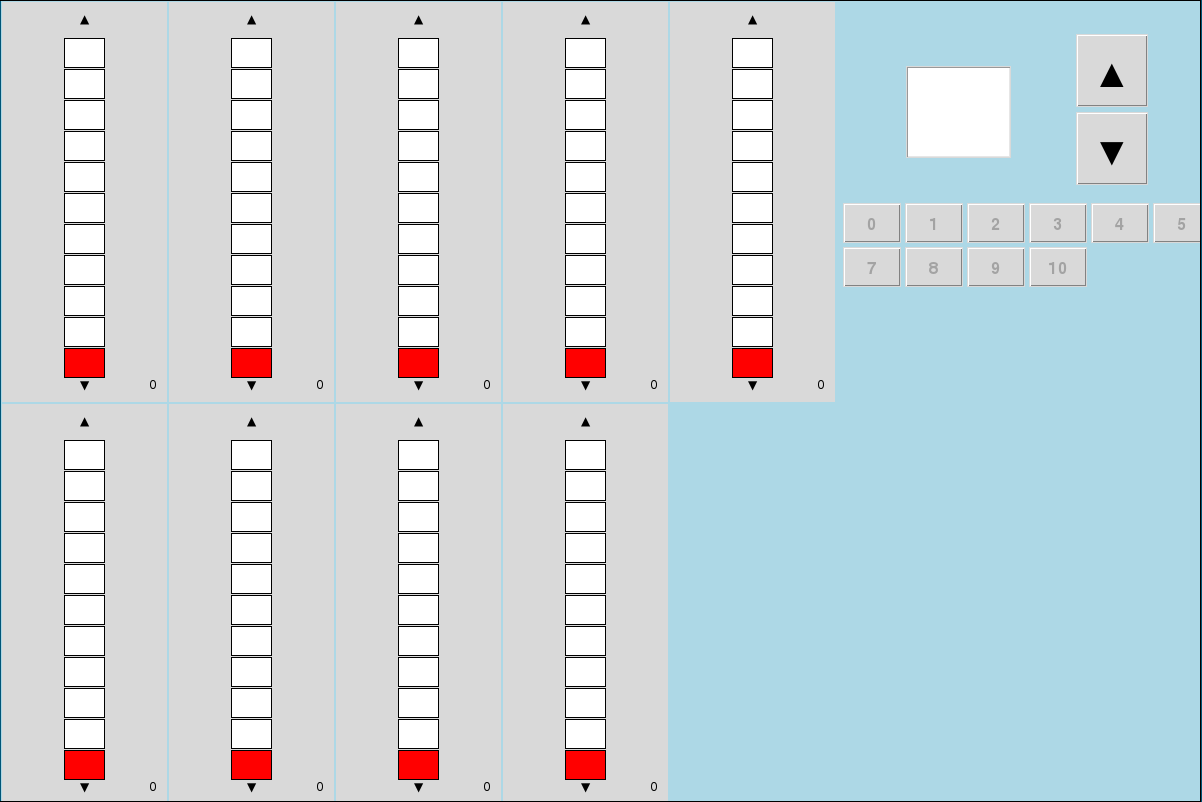
\includegraphics[width=0.93\textwidth]{img/winda.png}
	\end{figure}

\subsection{Controller}
Controller algorithm and program is to be developed.

\subsection{Connection}
Connection is based on simple sockets. Incoming port for controller is a the same time outcoming port for simulation program. On the other hand outcoming port for controller is an incomming port for simulation.
\newline
\newline
For now:
\newline
controller -\textgreater simulation is realised on port 8089,
\newline
simulation -\textgreater controller is realised on port 8090.

\subsection{Protocol}
Protocol coredpondes to events devindd in previous section.

\subsubsection{Controller \(\to\) Simulation commands}
\begin{enumerate}
	\item $X:Y$ (where X is number of elevator, Y is number of floor) - let elevator X move to floor Y.
	\item $X:s$ (where X is number of elevator) - let elevator X stops.
	\item $X:o$ (where X is number of elevator) - let elevator X opens the door.
	\item $X:c$ (where X is number of elevator) - let elevator X closes the door
\end{enumerate}


\subsubsection{Simulation \(\to\) Controller commands}
\begin{enumerate}
	\item $X:a$ (where X is number of elevator) - elevator X confirms execution of previous controller command.
	\item $Y:d$ (where Y is number of floor) - on the floor Y$^{th}$ user push the button to go down.
	\item $Y:u$ (where Y is number of floor) - on the floor Y$^{th}$ user push the button to go up.
	\item $X:Y$ (where X is number of elevator, Y is number of floor) - inside elevator X user push the button to go to the Y$^{th}$ floor.
\end{enumerate}	

Command $X:a$ should be send from simulation to controller after execution of any controller command. It provides a synchronization between both programs.

\end{document}
